\beginsong{Der Tod und der Mediziner}[mel={August Harder, ca. 1810}, txt={Gotthold Ephraim Lessing, 1747}, bo={168}, pfii={124}, pfiii={38}, gruen={167a}, kssiv={20}, index={Gestern Brüder könnt ihr‘s glauben, Tod und Mediziner}]

\beginverse 
\endverse
\centering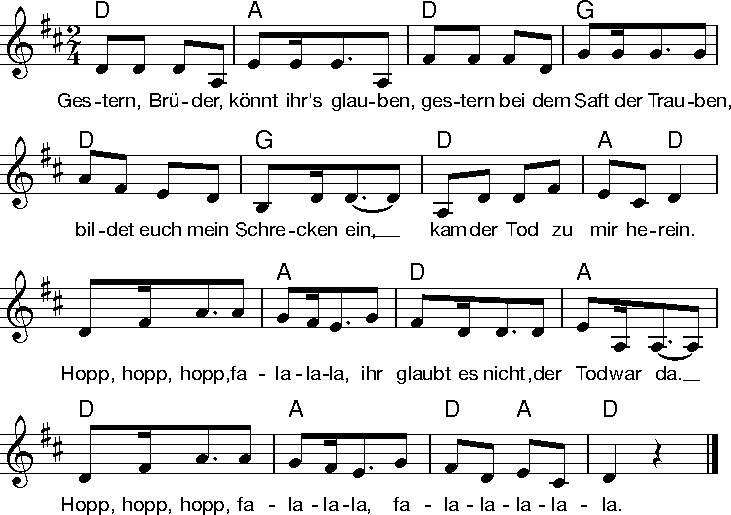
\includegraphics[width=1\textwidth]{Noten/Lied020.pdf}	

\beginverse\memorize
\[D]Drohend schwang er \[A]seine Hippe, \[D]drohend sprach das \[G]Furchtgerippe:
\[D]''Fort, du treuer \[G]Bacchusknecht! \[D]Fort, du hast ge\[A]nug ge\[D]zecht!''
\[D]''Lieber Tod'', sprach \[A]ich mit Tränen, \[D]''solltest du dich \[G]nach mir sehnen,
\[D]siehe, da steht \[G]Wein für dich. \[D]Lieber Tod, ver\[A]schone \[D]mich!''
\endverse

\beginchorus
\[D]Hopp, hopp, hopp, fa-\[A]la-la-la, ihr \[D]glaubt es nicht: Der \[A]Tod war da.
\[D]Hopp, hopp, hopp, fa-\[A]la-la-la, fa-\[D]la-la-\[A]la-la-\[D]la.
\endchorus


\beginverse
^Lächelnd greift er ^nach dem Glase, ^lächelnd trinkt er's ^aus der Base
^Auf der Pest Ge^sundheit leer, ^lächelnd stellt er's ^wieder ^her.
^Fröhlich glaubt' ich ^mich befreit, ^als er schnell sein ^Droh'n erneuert:
^''Narre, für ein ^Gläschen Wein ^denkst du'', sprach er, ^''los zu ^sein?''
\endverse
\renewcommand{\everychorus}{\textnote{\bf Refrain (wdh.)}}
\beginchorus
\endchorus

\beginverse
^''Tod'', sprach ich, ''ich ^möcht' auf Erden ^gern ein Medi^ziner werden.
^Lass mich, ich ver^spreche dir ^meine Kranken ^halb da^für!''
^''Gut, wenn das ist, ^magst du leben'', ^ruft er. ''Nun sei ^mir ergeben!
^Lebe, bis du ^sattgeküsst ^und des Trinkens ^müde ^bist!''
\endverse

\beginchorus
\endchorus

\beginverse
^Oh, wie schön klingt ^das den Ohren? ^''Tod, du hast mich ^neu geboren!
^Dieses Glas voll ^Rebensaft, ^Tod, auf gute ^Brüder^schaft!''
^Ewig muss ich ^also leben, ^ewig denn dein ^Gott der Reben,
^ewig soll mich ^Lieb' und Wein, ^ewig Wein und ^Lieb' er^freu'n.
\endverse

\beginchorus
\endchorus

\endsong

\begin{intersong}
\ifthenelse{\boolean{pics}}{
    \ThisLRCornerWallPaper{0.35}{Bilder/TodUndMediziner_heiko.png}
}{}
\end{intersong}